\documentclass[12pt,a4paper]{article}

\usepackage[margin=22mm]{geometry}
\usepackage{fontspec}
\setmainfont{DejaVu Serif}
\usepackage{polyglossia}
\setdefaultlanguage{russian}
\usepackage{graphicx}
\usepackage{float}
\usepackage{amsmath}
\usepackage{enumitem}

\begin{document}
\sloppy

\begin{center}
    \Large\textbf{Алгоритм Кристофидеса-Сердюкова}
\end{center}

\section*{Постановка задачи}
Дан полный неориентированный граф $G=(V,E)$ с неотрицательными
весами рёбер $w(u,v)$. Веса симметричны
и удовлетворяют неравенству треугольника:
\[
    w(u,v)=w(v,u), \qquad
    w(u,v)+w(v,z)\geq w(u,z).
\]
Нужно найти гамильтонов цикл наименьшего веса, то есть
замкнутый маршрут, проходящий через каждую вершину ровно один раз.

\section*{Идея алгоритма}
Алгоритм строит приближённое решение метрической задачи
коммивояжёра с гарантией
\[
    w(C)\leq\frac32\,\mathrm{OPT},
\]
где $\mathrm{OPT}$ --- вес оптимального гамильтонова цикла.\\

Шаги алгоритма:
\begin{enumerate}[leftmargin=*,itemsep=2pt]
    \item Найти минимальное остовное дерево $T$.
    \item Выделить вершины нечётной степени в $T$.
    \item Построить минимальное совершенное паросочетание
          на выделенных вершинах.
    \item Объединить остов и паросочетание в мультиграф.
    \item Найти эйлеров цикл полученного мультиграфа.
    \item Вычеркнуть повторяющиеся вершины, опираясь на неравенство треугольника.
    \item Вернуть полученный гамильтонов цикл.
\end{enumerate}

\section*{Пример работы}
Рассмотрим полный граф с четырьмя вершинами: $A$, $B$, $C$, $D$.

\begin{figure}[H]
    \centering
    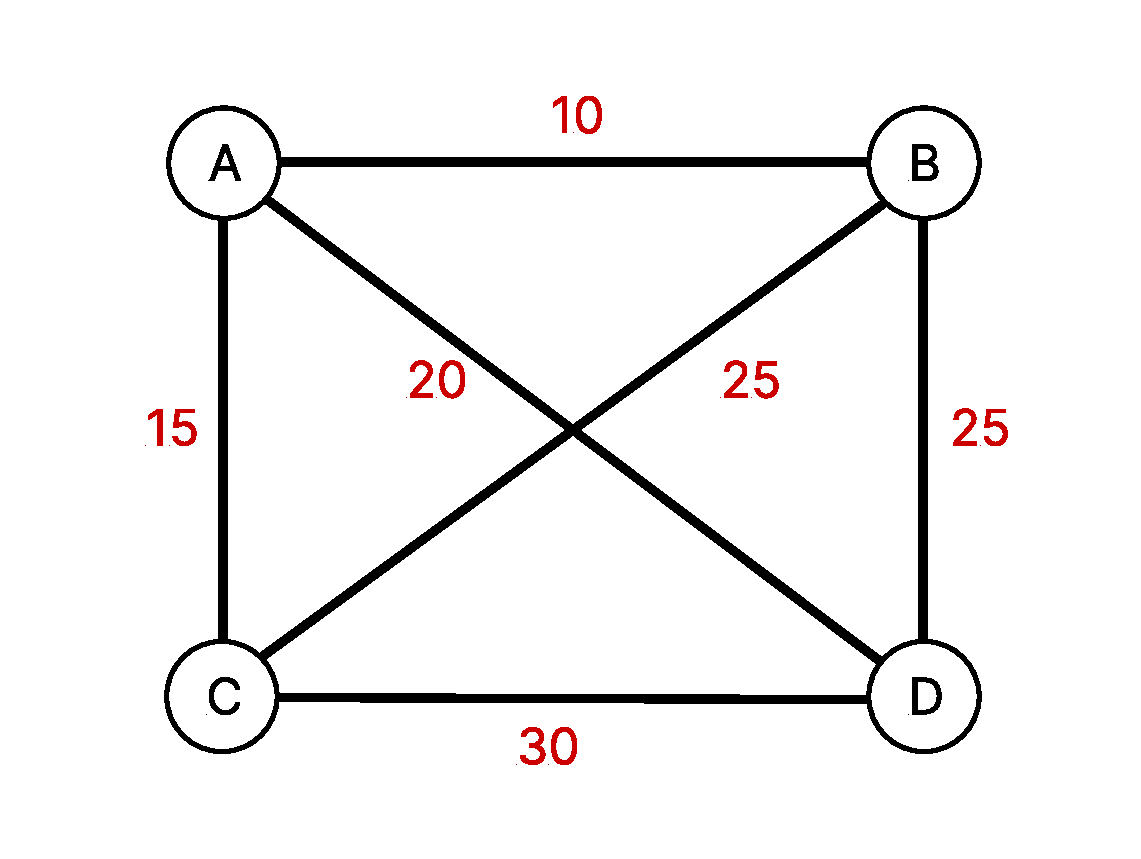
\includegraphics[width=0.55\textwidth]{figures/graph.pdf}
    \caption{Исходный граф.}
\end{figure}

Построим по нему минимальный остов. Он содержит рёбра $AB$, $AC$, $AD$.
Его вес: $10+15+20=45$.
Все четыре вершины имеют нечётную степень: $R=\{A,B,C,D\}$.

\begin{figure}[H]
    \centering
    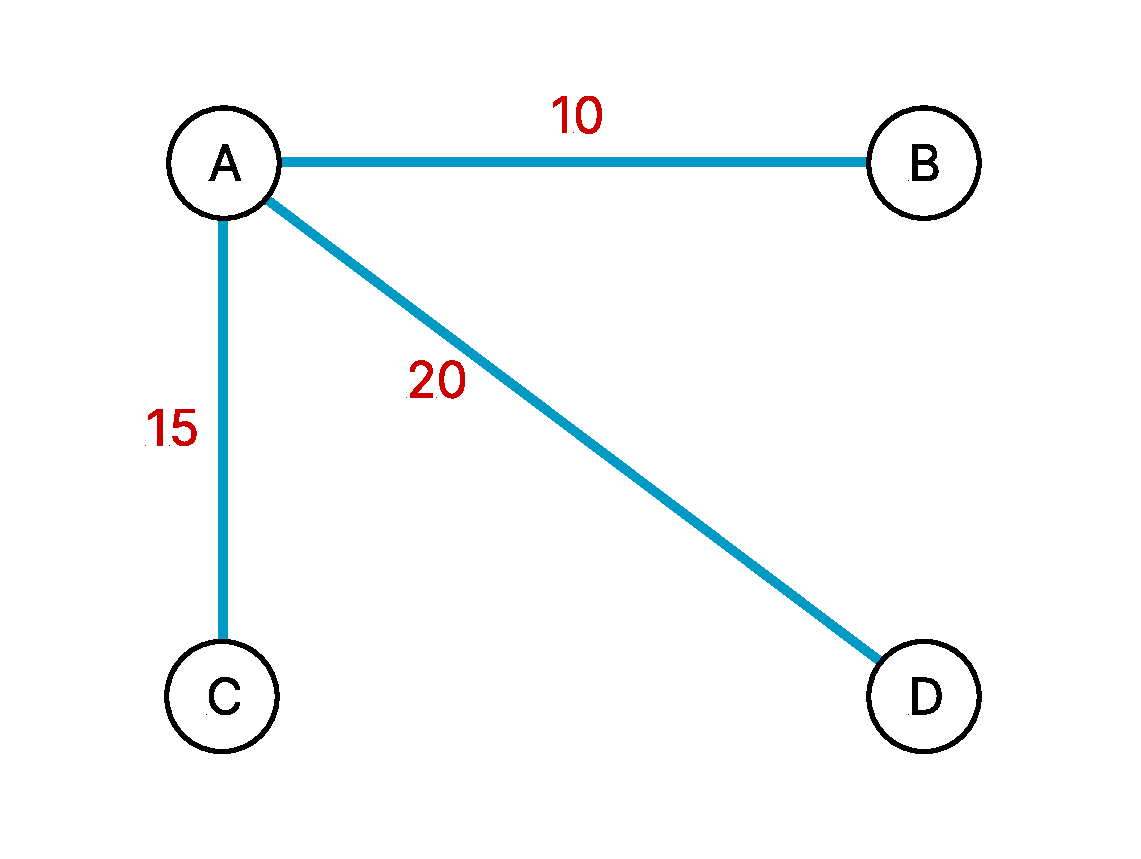
\includegraphics[width=0.55\textwidth]{figures/tree.pdf}
    \caption{Минимальное остовное дерево.}
\end{figure}

Далее построим минимальное совершенное паросочетание
$M=\{AB,CD\}$ веса $10+30=40$.
Другое минимальное паросочетание $\{AC,BD\}$ также имеет вес $40$, берем любое.
После объединения с остовом получаем мультиграф, где все вершины имеют четную степень, из чего следует, что граф эйлеров.
Красным пунктиром показаны дополнительные рёбра паросочетания (кратные ребра сохраняются).

\begin{figure}[H]
    \centering
    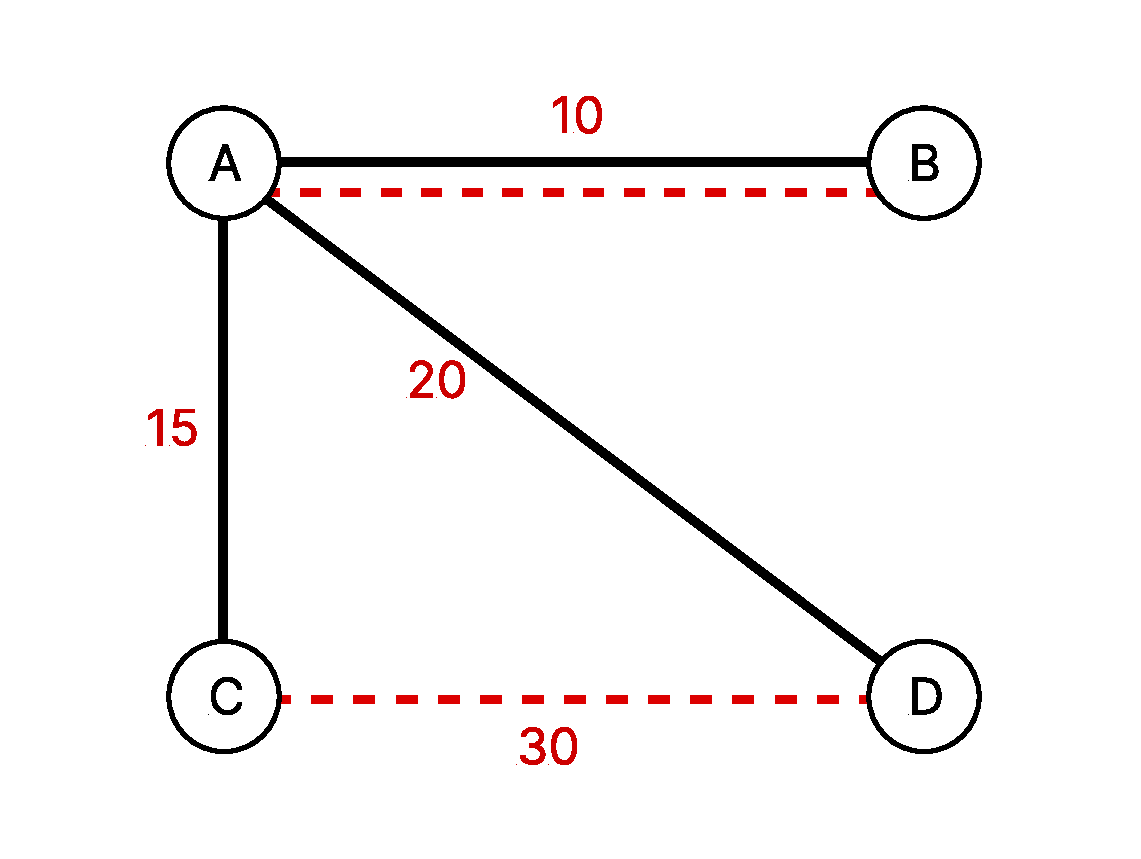
\includegraphics[width=0.55\textwidth]{figures/multigraph.pdf}
    \caption{Остов и минимальное паросочетание.}
\end{figure}

Один из эйлеровых циклов:
\[
   A\to B\to A\to C\to D\to A.
\]
Его вес равен $10+10+15+30+20=85$.
Далее для гамильтонова цикла исключим повторные вершины, пройдя прямым путем, используя неравенство треугольника ($B\to A\to C \geq B\to C$). Пропустив повторную вершину $A$, получим цикл
$A\to B\to C\to D\to A$.

\begin{figure}[H]
    \centering
    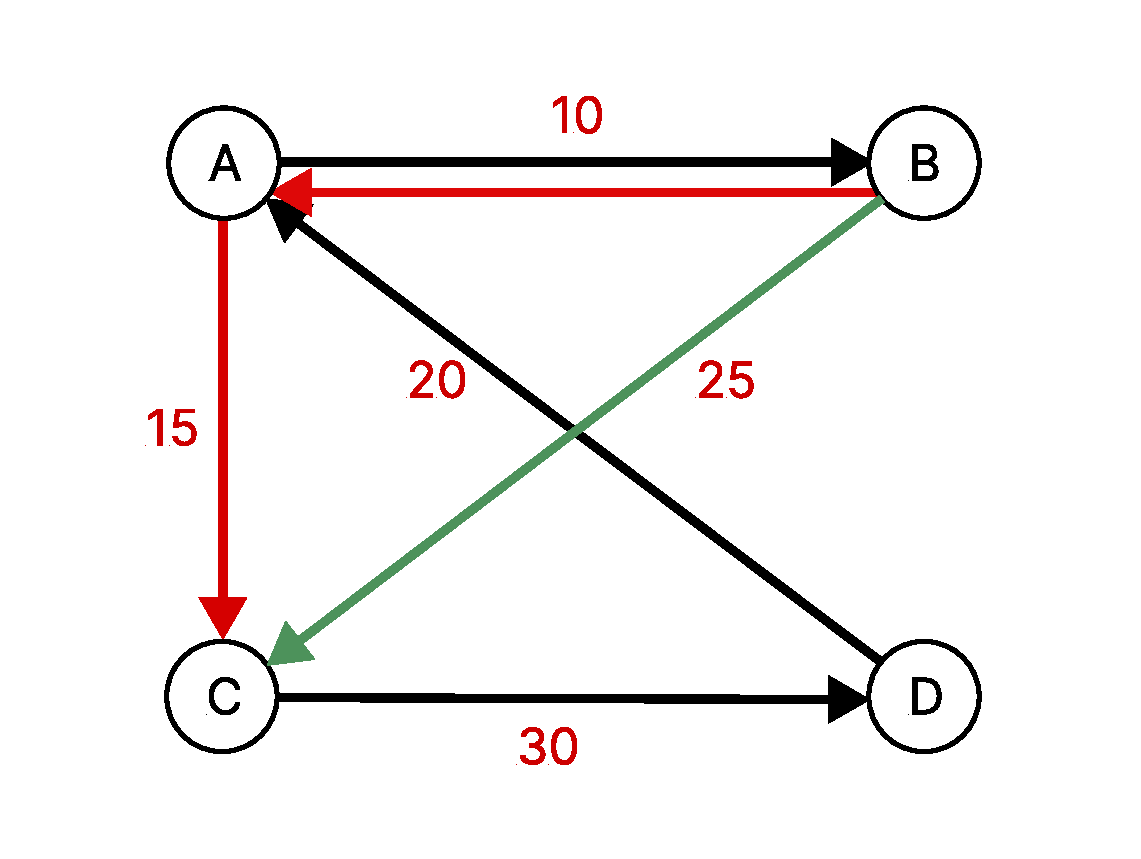
\includegraphics[width=0.55\textwidth]{figures/el_cycle.pdf}
    \caption{Построение гамильтонова цикла по эйлерову циклу.}
\end{figure}

\begin{figure}[H]
    \centering
    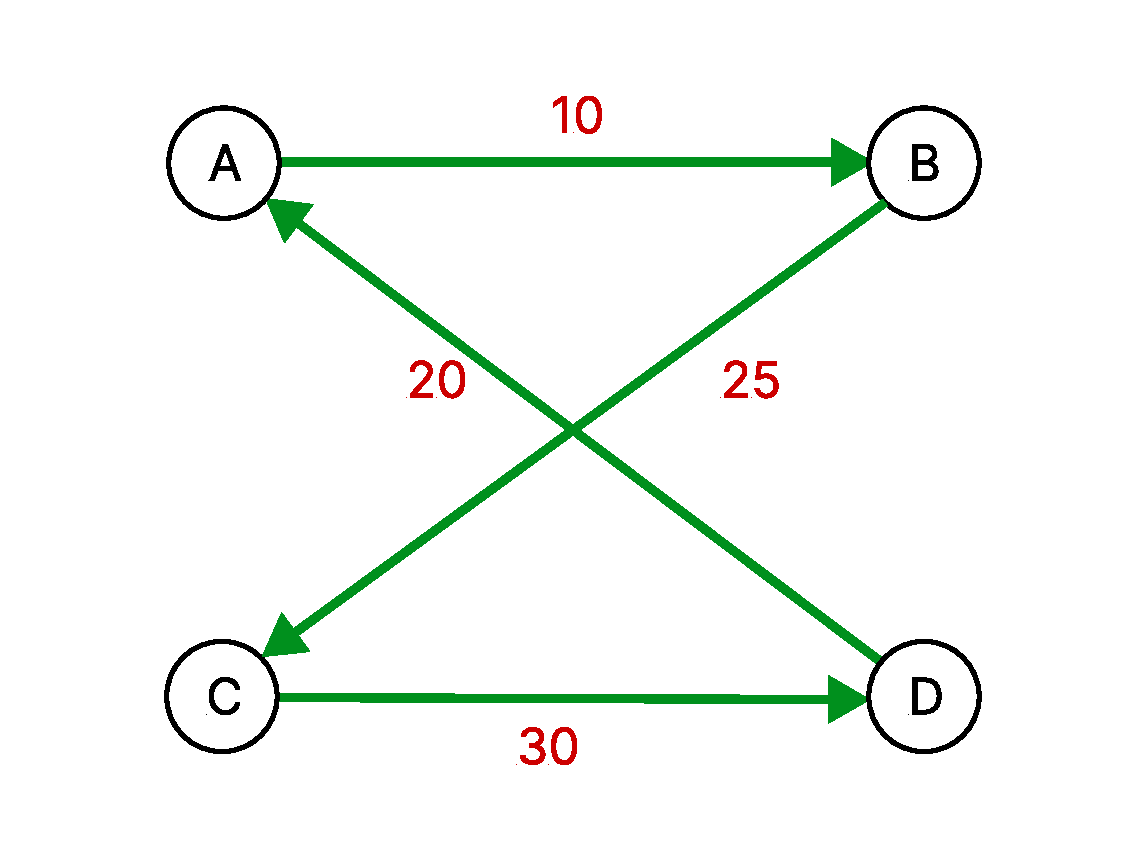
\includegraphics[width=0.55\textwidth]{figures/cycle.pdf}
    \caption{Полученный гамильтонов цикл.}
\end{figure}

\section*{Результат}
Вес построенного цикла:
\[
    w(C)=10+25+30+20=85.
\]
Для данного графа оптимальный цикл
$A\to B\to D\to C\to A$ имеет вес
\[
    \mathrm{OPT}=10+25+30+15=80.
\]
Гарантия алгоритма выполняется:
\[
    85\leq\frac32\cdot80=120.
\]
Таким образом, построен гамильтонов цикл с весом,
не превышающим $3/2$ от оптимального.


\section*{Обоснование оптимальности приближённого решения}

Покажем, что вес цикла, построенного алгоритмом
Кристофидеса--Сердюкова, не превышает
$\frac{3}{2}$ от веса оптимального решения.
Обозначим \\\\через $\mathrm{OPT}$ вес оптимального
гамильтонова цикла,\\ через $T$ --- минимальное
остовное дерево,\\ а через $M$ --- минимальное
совершенное паросочетание нечётных вершин.\\\\
Если удалить одно ребро из оптимального цикла,
получится остовное дерево. Поэтому вес
минимального остова не больше оптимума:
\[
    w(T) \leq \mathrm{OPT}.
\]

Теперь оценим вес паросочетания.\\ Рассмотрим
нечётные вершины дерева $T$ в том порядке,
в котором они встречаются в оптимальном цикле.
Их количество чётно (по лемме о рукопожатиях). Разделим полученный
замкнутый маршрут на два паросочетания,
соединяя соседние нечётные вершины поочерёдно.
По неравенству треугольника суммарный вес
этих двух паросочетаний не превышает
$\mathrm{OPT}$. Значит, хотя бы одно из них
имеет вес не больше $\mathrm{OPT}/2$.
Поскольку алгоритм выбирает минимальное
паросочетание, получаем:
\[
    w(M) \leq \frac{1}{2}\mathrm{OPT}.
\]

После объединения остова и паросочетания
получается эйлеров мультиграф. Вес его
эйлерова цикла равен $w(T)+w(M)$.
При удалении повторных посещений вершин
вес маршрута не увеличивается благодаря
неравенству треугольника. Следовательно,
для полученного гамильтонова цикла $C$
выполняется:
\[
    w(C) \leq w(T)+w(M)
    \leq \mathrm{OPT}+\frac{1}{2}\mathrm{OPT}
    = \frac{3}{2}\mathrm{OPT}.
\]

Таким образом, алгоритм гарантирует
приближённое решение, вес которого
не более чем в $1{,}5$ раза превышает
оптимальный.

\section*{Источники}

\begin{enumerate}[leftmargin=*,itemsep=2pt]
    \item Алгоритм Эдмундса по паросочетаниям.
\end{enumerate}

\end{document}
